\section{Results}

\subsection{Qualitative}

We present findings in relation to six NASSS domains: (1) the condition, (2) the technology, (3) the value proposition, (4) the intended adopters, (5) the healthcare organisation, and (6) the wider system.

\subsubsection{Domain 1: The condition}

Physicians emphasised the heterogeneous and complex nature of the presentation of patients with stroke. They frequently used the concept ‘barn door’ to refer to a situation when a patient was perceived to be presenting with ‘classic’ symptoms of ischaemic stroke and where guidelines for treatment with thrombolysis could easily be followed and decision-making was straight-forward. However, physicians suggested most patients were not ‘barn-door’ presentations (also known as \textit{clinical grey areas}), making decisions regarding thrombolysis more challenging.

Clinicians stressed the complexity of decision-making with respect to thrombolysis, particularly in clinical grey areas, and the perceived level of risk involved in the procedure. They discussed weighing up the risks/benefits in each case and challenges of obtaining informed consent for thrombolysis.

Clinicians characterised themselves and colleagues as pro or anti-thrombolysis, or keen or reluctant thrombolysers, the latter typically because they had experience of negative patient outcomes following thrombolysis and/or were generally more risk averse. Some reservations were also expressed about targets to improve thrombolysis rates.

\subsubsection{Domain 2: The technology}

Participants from one of the sites emphasised the necessity of the SAMueL-2 technology incorporating data on the configuration of acute stroke services for it to be seen as having validity. Most participants expressed having trust and confidence in SSNAP data and some referred to its potential to improve stroke services, but not all understood or engaged with the programme and thus were unsure how machine learning from SSNAP data could improve thrombolysis decision-making. Others were more enthusiastic about the potential for machine learning to extend the utility of SSNAP as a learning system for quality improvement. The addition of machine learning to the SSNAP portal was mooted as improving its sensitivity and potential for quality improvement vis-à-vis thrombolysis.

Some clinicians discussed their current use of AI based systems such as Brainomix or RapidAI and showed interest in SAMueL-2 becoming interoperable with these systems. Others expressed scepticism.

\subsubsection{Domain 3: The value proposition}

Reporting in this NASSS domain focusses on perceived demand-side value (while perceived supply-side value is reported as part of Domain 6 ‘The Wider System’). SAMueL-2 can be characterised as being at the value promise \textit{developmental} stage; our data reflects the perceived or anticipated value of the technology which is relatively speculative.

SAMueL-2 was seen by some as providing the potential to address variation in clinical practice between clinicians and across trusts. Many participants perceived value in the potential for machine learning to help them in clinical grey areas when decision-making was most difficult, but there was uncertainty and ambivalence regarding whether this would/could happen during the acute stroke pathway. They hoped the SAMueL-2 technology would provide more specific and objective assessments of risk/benefit of the procedure and inform consent discussions. Some perceived it to be inevitable that AI/machine learning would eventually be used in real-time at the point of care. Some clinicians saw the value of the web app benchmarking feature to change culture or local thrombolysis guidelines. However, it was emphasised that this benchmarking should include data on patient complications and outcomes for it to be seen as valid and useful.

Participants discussed the perceived utility of the SAMueL-2 technology as a ‘learning tool’ to review clinical cases and provide training or quality assurance, for example at governance meetings. It was perceived as being useful as a decision-aid for trainees, non-stroke specialists and at district general hospitals.

\subsubsection{Domain 4: The intended adopters}

Some ED physicians were less confident about the evidence base for thrombolysis. They expressed a lack of faith in the clinical trials and reluctance to thrombolyse due to perceived risks of the procedure. One said they preferred thrombectomy to thrombolysis because they perceived that thrombectomy had more robust evidence to support it and fewer risks associated with it.

Some interviewees asserted that the web app benchmarking feature was not suitable or useful for experienced consultants like themselves, emphasising trust in their own clinical acumen. Others worried about how benchmarking and comparison might be used and were anxious about how it might affect them. Concern was also expressed that AI might be given primacy over clinical decision-making and that this could adversely affect patient outcome.

\subsubsection{Domain 5: The healthcare organisation}

Participants discussed recent successful quality improvement initiatives regarding stroke, for example, improvement in door-to-needle times. For example, site A had initiated a stroke quality improvement week, and Site B had undertaken a reconfiguration of the acute stroke pathway which involved new stroke nurse assessor roles and stroke healthcare assistants. Each team member had been designated specific tasks facilitating speed of the acute pathway. Most participants at site B felt confident in the acute stroke processes and that there was readiness for organisational change. One participant suggested that there was potential for experienced non-consultant level staff to thrombolyse without a consultant being present to speed up the process.

However, participants also described organisational-level barriers they perceived to be impeding thrombolysis provision, such as:

\begin{itemize}
    \item inexperienced clinical leadership

    \item workforce shortages and lack of specialist and experienced stroke nurses

    \item bureaucracy

    \item limited availability of imaging

    \item a culture that doesn't support use of thrombolysis

    \item funding constraints

    \item lack of access to computers

    \item overcrowding

\end{itemize}

Some people were enthusiastic that SAMueL-2 technology could be instrumental in overcoming these institutional barriers.

\subsubsection{Domain 6: The wider system}

Our analysis indicated that the wider professional and political context was important for adoption and scale-up of SAMueL-2. Stakeholders and participants from ISDNs were, with some expressed reservations about usability of the SSNAP interface, enthusiastic about SAMueL-2 being added to the portal and about facilitating its roll out to and uptake by sites for quality improvement.

The development of machine learning in conjunction with SSNAP was referred to by one national level policymaker as offering “the prospect of contributing significantly to reductions in stroke-related disability” [stakeholder communication] and was seen as having relevance to the NHS Long Term Plan. This appears to constitute a clear supply-side value proposition. The TASC initiative provided a ‘policy push’ for SAMueL-2 technology implementation, albeit initially on a limited scale.

Key findgings:

\begin{itemize}
    \item Participants were hopeful the SAMueL-2 technology could address variance in thrombolysis practice. It was seen as particularly suitable for junior clinicians, non-stroke specialists and at district general hospitals and offered value for training, reviewing clinical cases, and quality improvement.

    \item Given reservations expressed about the underpinning SSNAP data, it is important to reassure intended adopters about the integrity of modelling based on this data.

    \item Evidence indicated that emergency department physicians may have less confidence in the evidence base for thrombolysis.

    \item Perceived lack of funding and stroke workforce shortages may impede quality improvement and adoption of new technologies such as SAMueL-2

\end{itemize}




\subsection{Quantitative: Thrombolysis use}

\begin{enumerate}
    \item Thrombolysis use in patients arriving within 4 hours of known or estimated stroke onset ranged 7\% to 49\% between hospitals.

    \item The odds of receiving thrombolysis reduced 9-fold over the first 120 minutes of arrival-to-scan time, varied 30-fold with stroke severity, reduced 3-fold with estimated rather than precise stroke onset time, reduced 6-fold with increasing pre-stroke disability, reduced 4-fold with onset during sleep, reduced 5-fold with use of anticoagulants, reduced 2-fold between 80 and 110 years of age, reduced 3-fold between 120 and 240 min of onset-to-arrival time and varied 13-fold between hospitals.
    
    \item The majority of between-hospital variance was explained by the hospital, rather than by the differences in local patient populations.
\end{enumerate}


\begin{figure}
    \centering
    \begin{subfigure}{0.8\textwidth}
      \centering
      \captionsetup{width=.9\linewidth}
      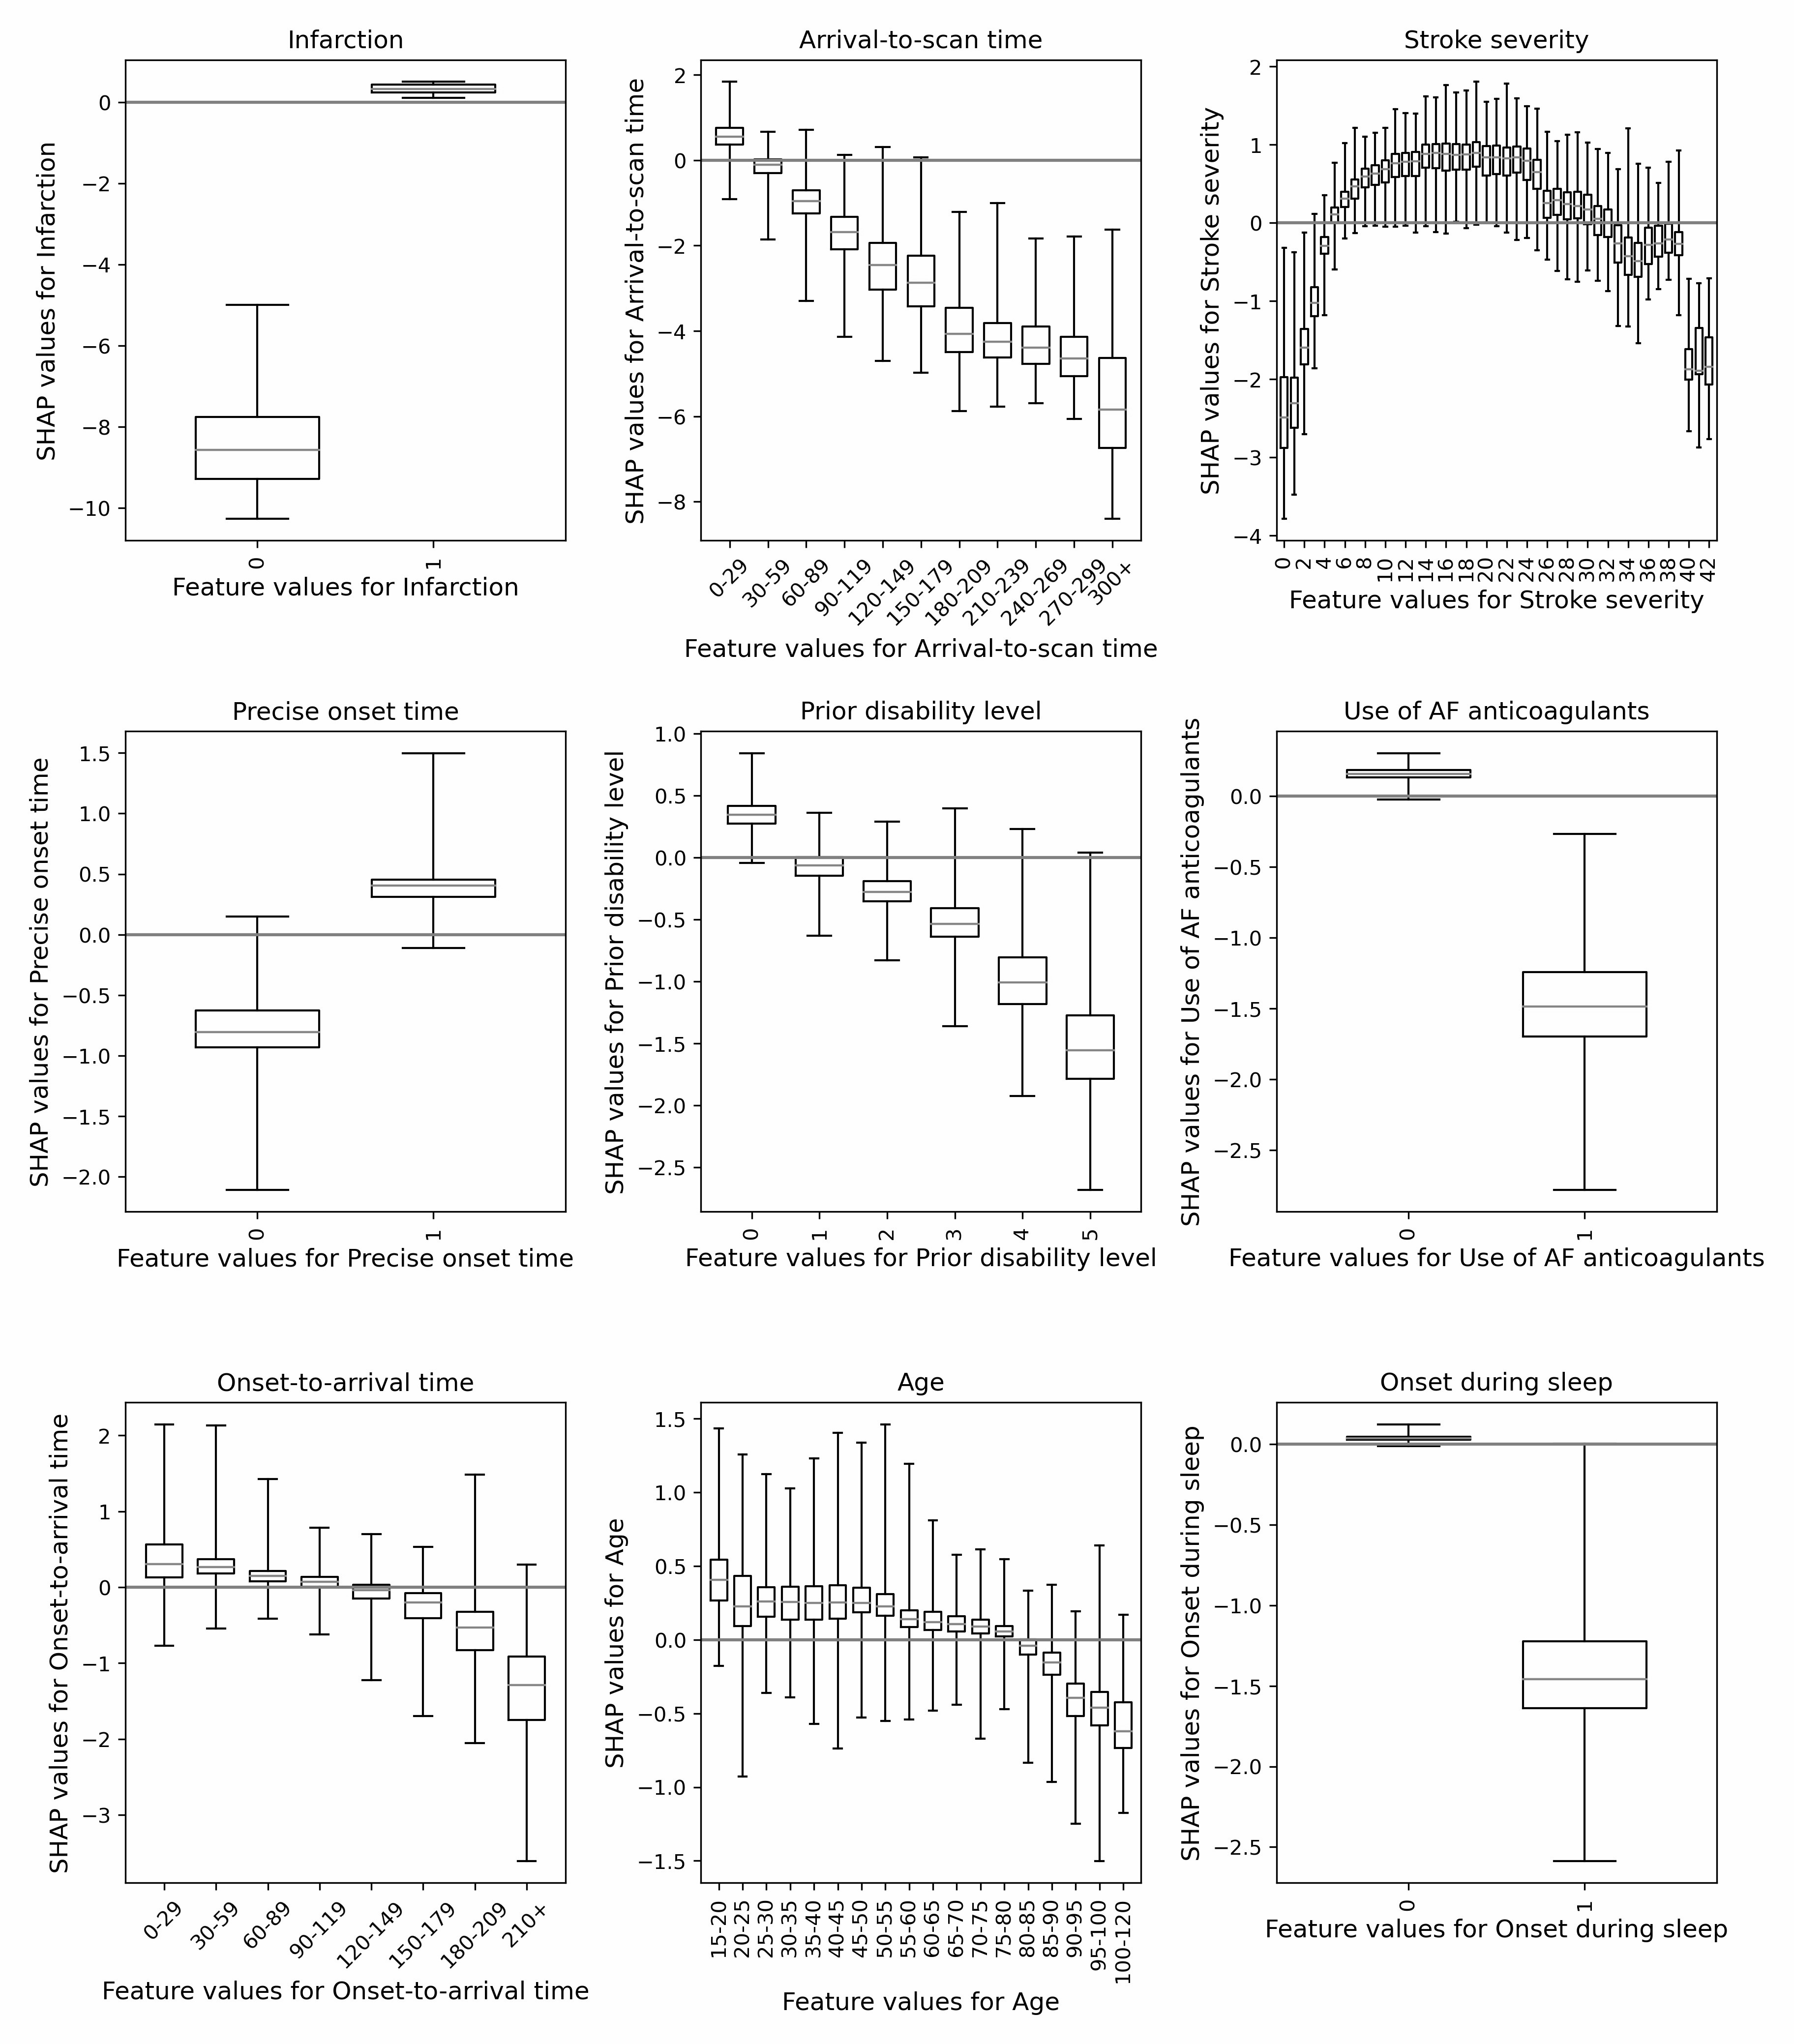
\includegraphics[trim={0 0 0 1.2cm}, clip, width=0.95\linewidth]      {images/p2_patient_shap.jpg}\\
        \caption{Box plots showing the relationship between SHAP values and feature values. Box plots show inter-quartile range (box), median (mid-line in box), and range (whiskers). The plots are ordered in ranked feature importance (using the mean absolute SHAP value across all instances).}
        \label{fig:global_shap}
    \end{subfigure}
    \hfill
    \begin{subfigure}{0.8\textwidth}
      \centering
      \captionsetup{width=.9\linewidth}
      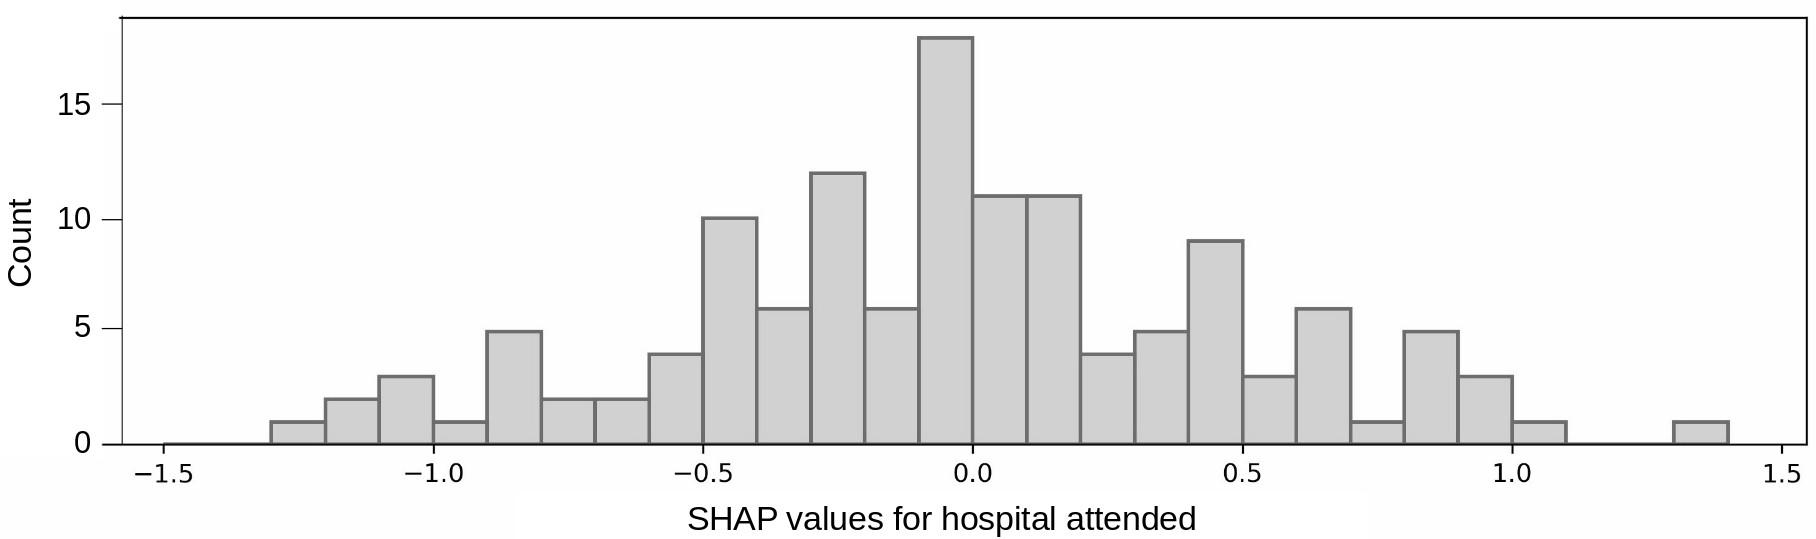
\includegraphics[trim={0 0 0 0.1cm}, clip, width=1\linewidth]    {images/p2_hosp_shap.jpg}
    \caption{Histogram showing the frequency of SHAP values for the hospital attended.}
    \label{fig:hospital_shap}
    \end{subfigure}

  \caption{Plots showing the relationship between SHAP values and feature values for predicting thrombolysis use. Top: Violin plots showing the relationship between SHAP values and feature values. The horizontal line shows the median SHAP value. Bottom: Histogram showing the frequency of the mean SHAP value for the hospital attended.}
    \label{fig:shap_outcome_model}
\end{figure}



%%%%%%%%%%%%%%%%%%%%%%%%%%%%%%%%%%%%%%%%%%%%%%%%%%%
\subsection{Quantitative: Patient clinical outcome}


\subsection{Influences on best and worst outcomes across a patient cohort}

In order to understand general characteristics affecting outcomes, we have shown how patient feature values, and stroke team attended, affected the likelihood of having the best (mRS 0) or worst (mRS 6) outcomes (figure \ref{fig:shap_outcome_model}) across 15,680 test patients (which were not used to train the model). Feature values that contributed to the best outcome on discharge (mRS 0) were no prior disability, milder stroke, earlier thrombolysis, younger, no atrial fibrillation diagnosis, and precisely known stroke onset time. Feature values that contributed to the worst outcome on discharge (mRS 6) were higher prior disability, more severe stroke, later or no thrombolysis, older, diagnosis of atrial fibrillation, and an imprecisely known onset time. The hospital attended also affected outcome predictions, with a  larger contribution from the attended hospital contribution for mRS 0, rather than mRS 6, at discharge. 


\begin{figure}[h]
    \centering
    \begin{subfigure}{.5\textwidth}
      \centering
      \captionsetup{width=.9\linewidth}
      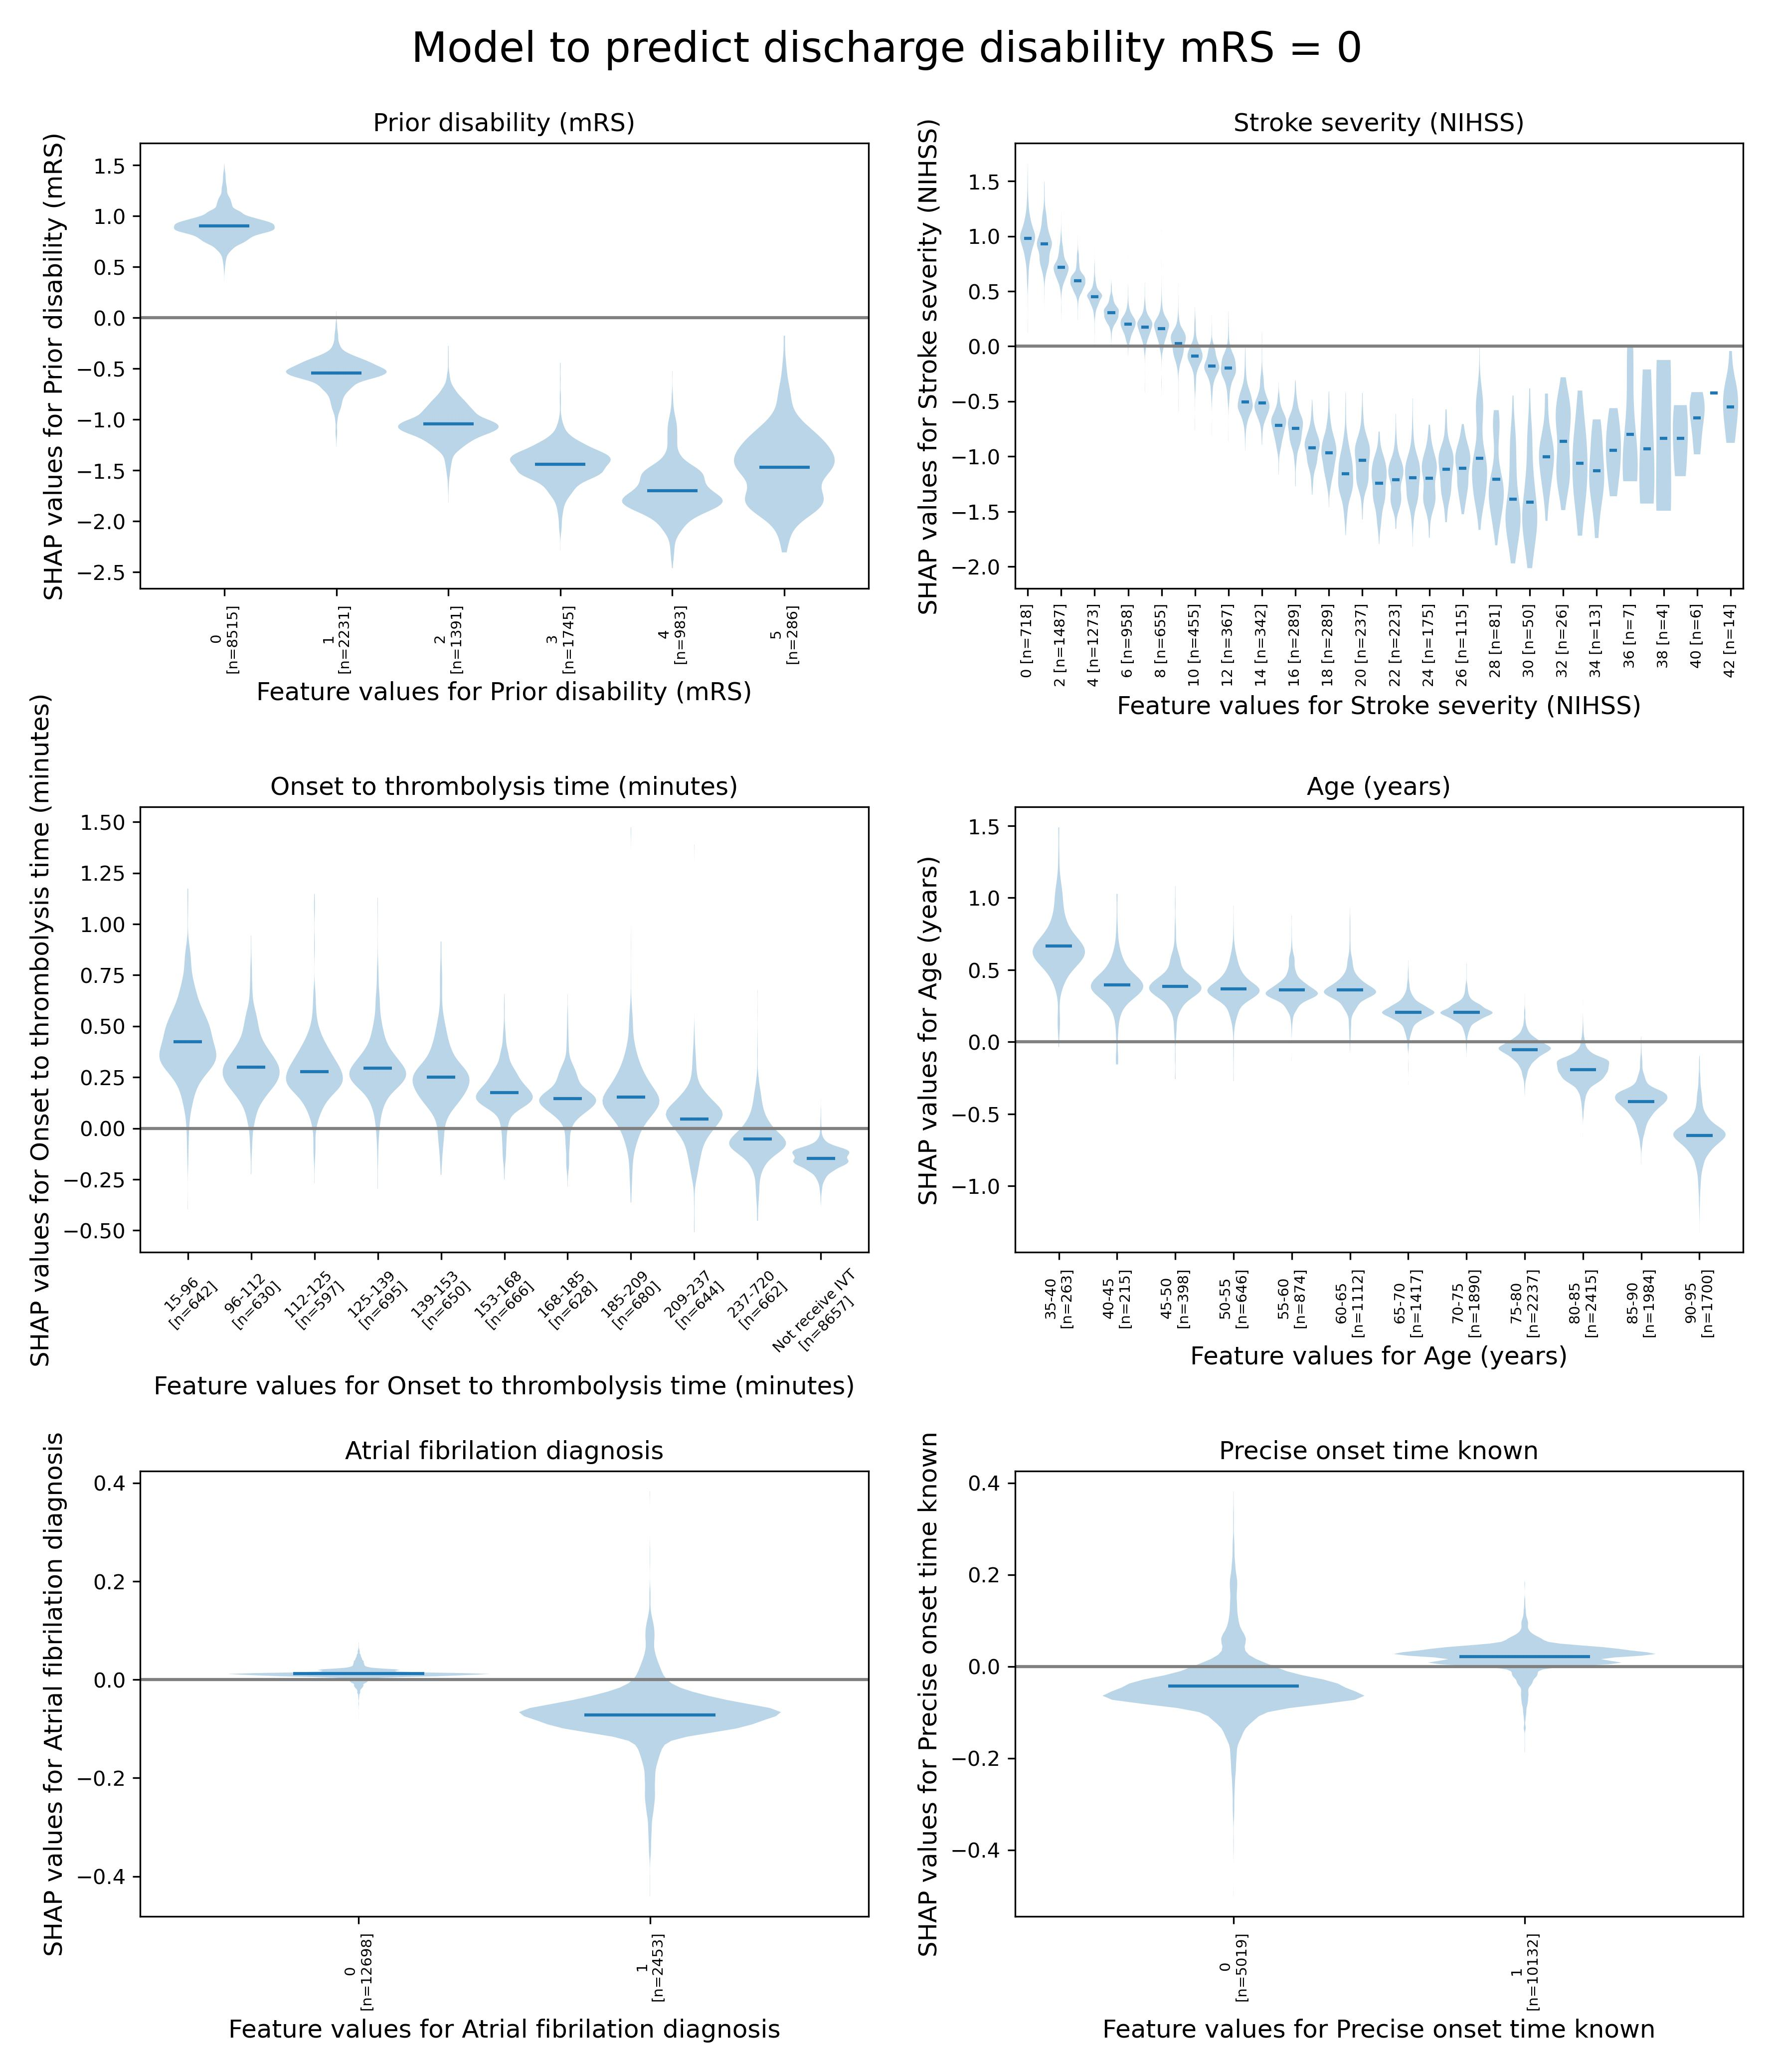
\includegraphics[trim={0 0 0 1.2cm}, clip, width=0.95\linewidth]      {./images/053_xgb_7_features_1fold_thrombolysis_shap_violin_all_features_for_mRS0}\\

    \end{subfigure}%ults
    \begin{subfigure}{.5\textwidth}
      \centering
      \captionsetup{width=.9\linewidth}
      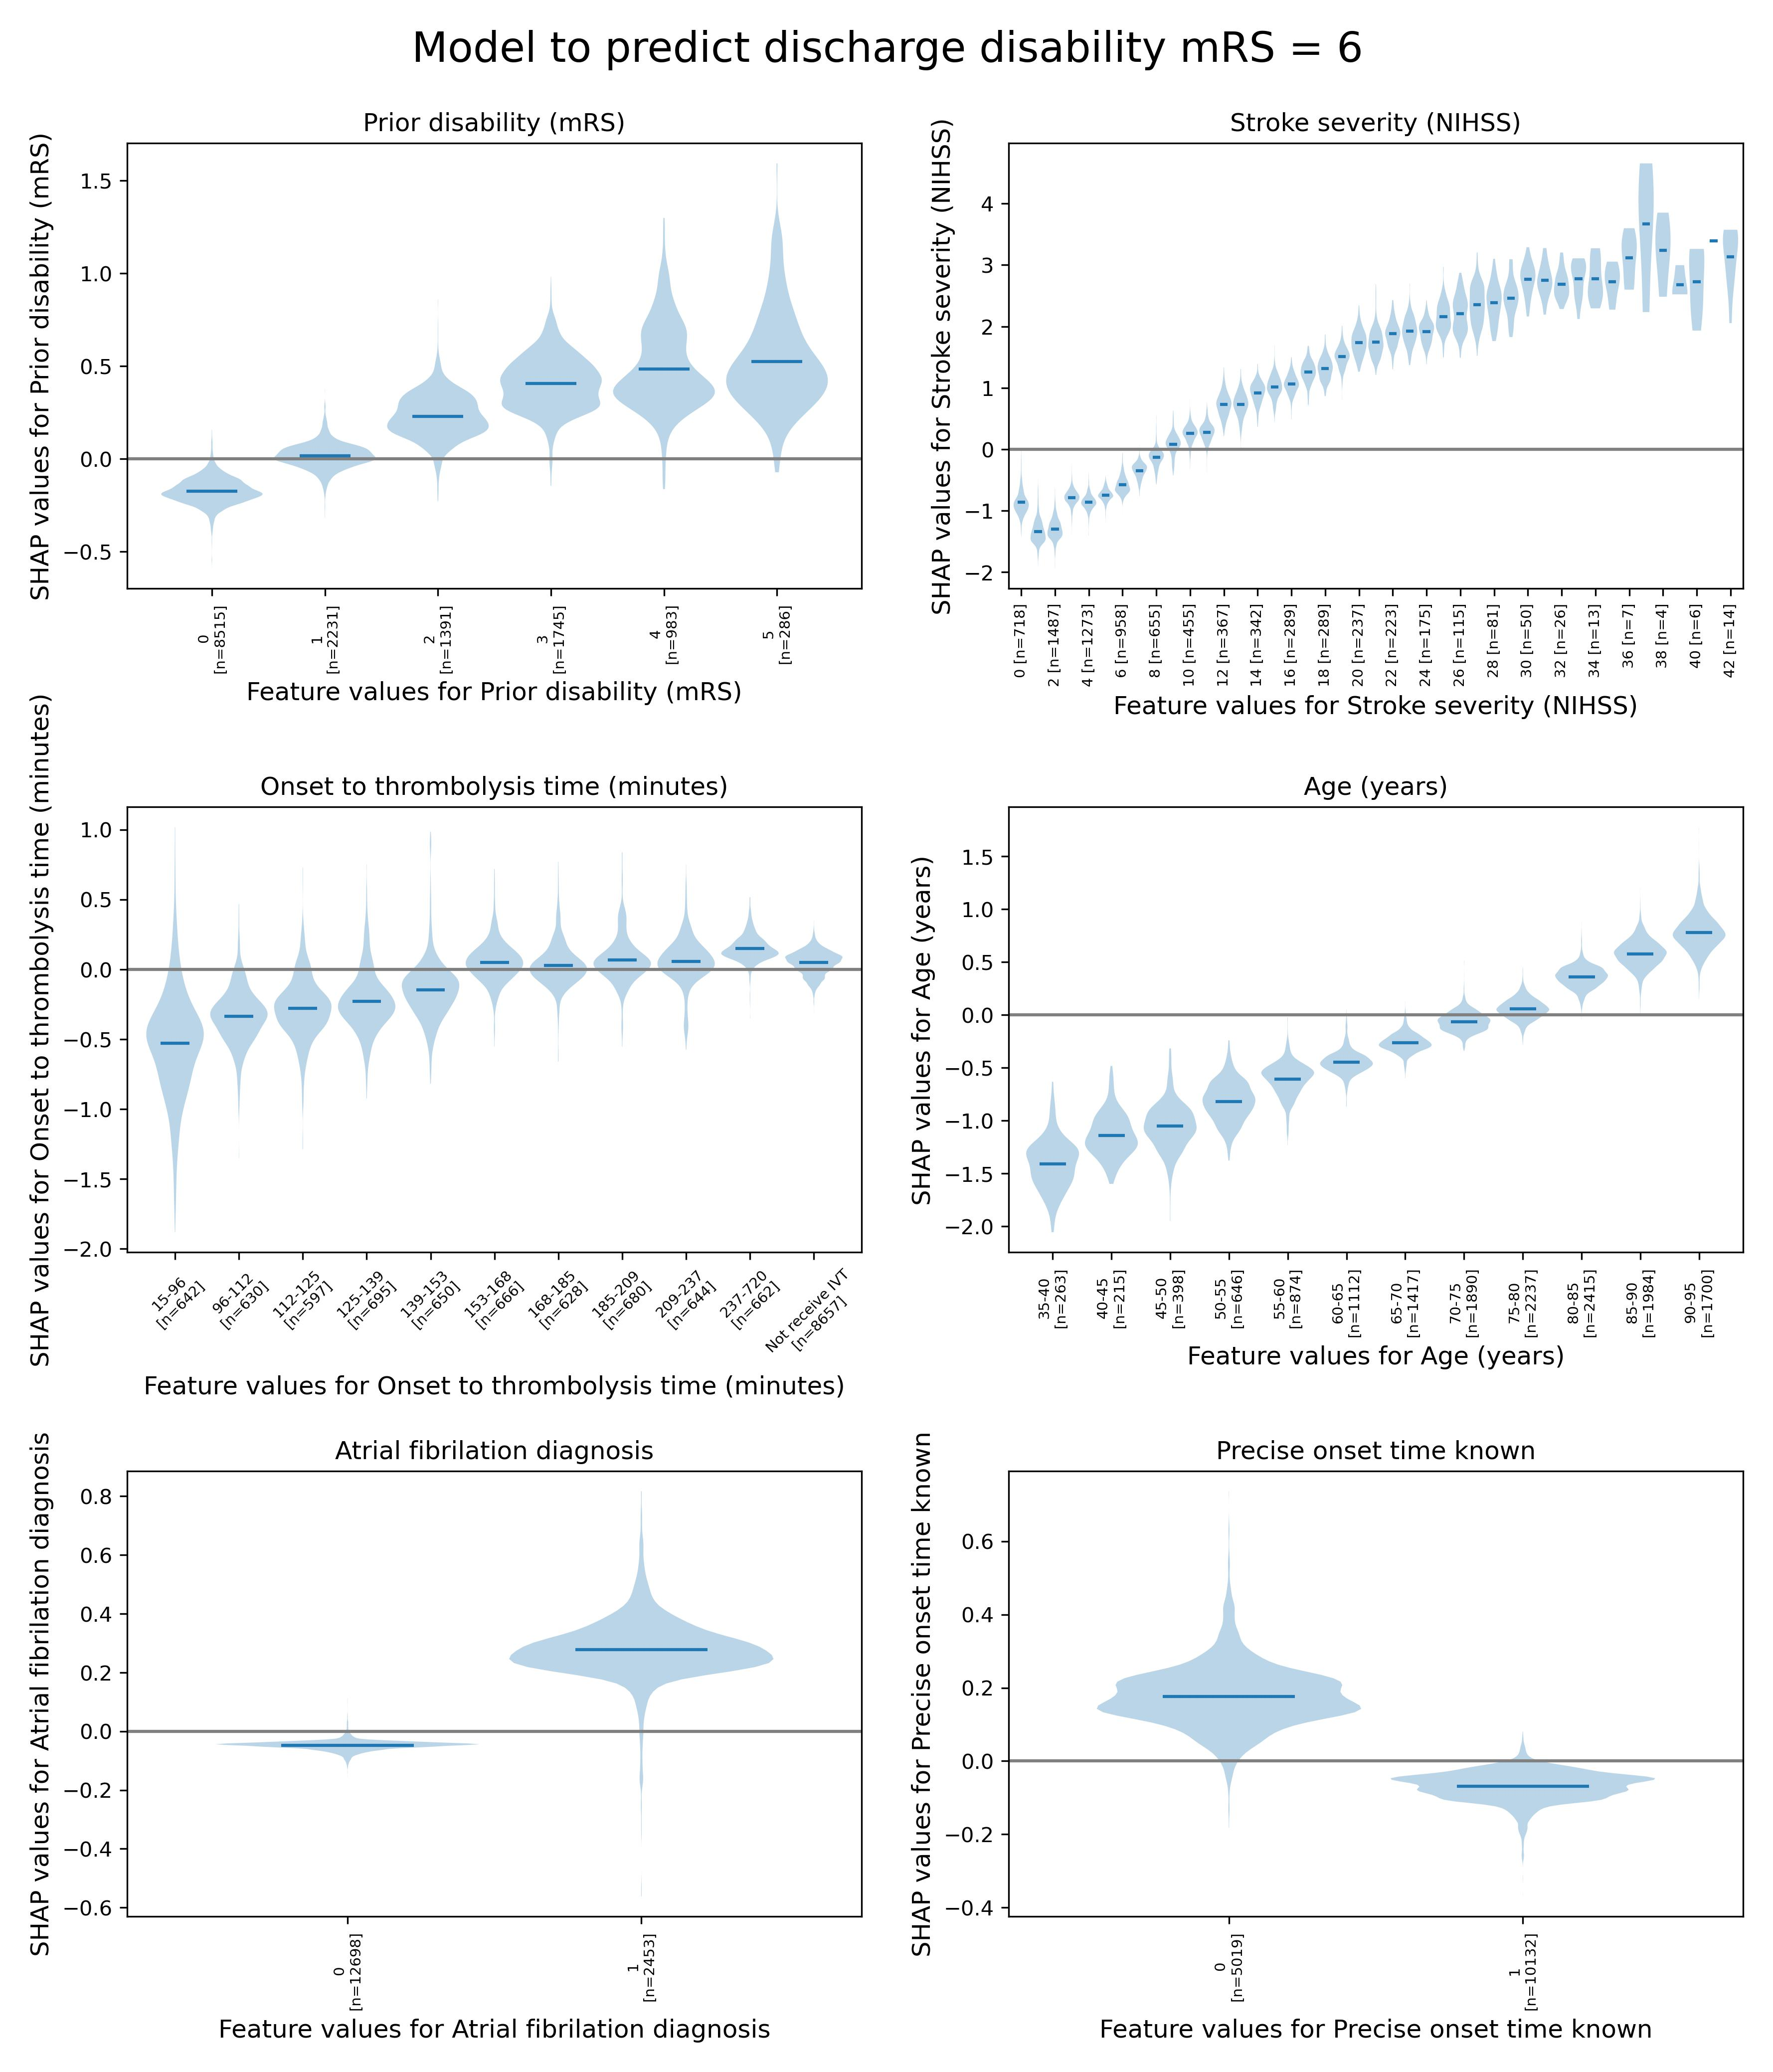
\includegraphics[trim={0 0 0 1.2cm}, clip, width=0.95\linewidth]      {./images/053_xgb_7_features_1fold_thrombolysis_shap_violin_all_features_for_mRS6}\\
    \end{subfigure}
    \hfill
    \begin{subfigure}{.5\textwidth}
      \centering
      \captionsetup{width=.9\linewidth}
      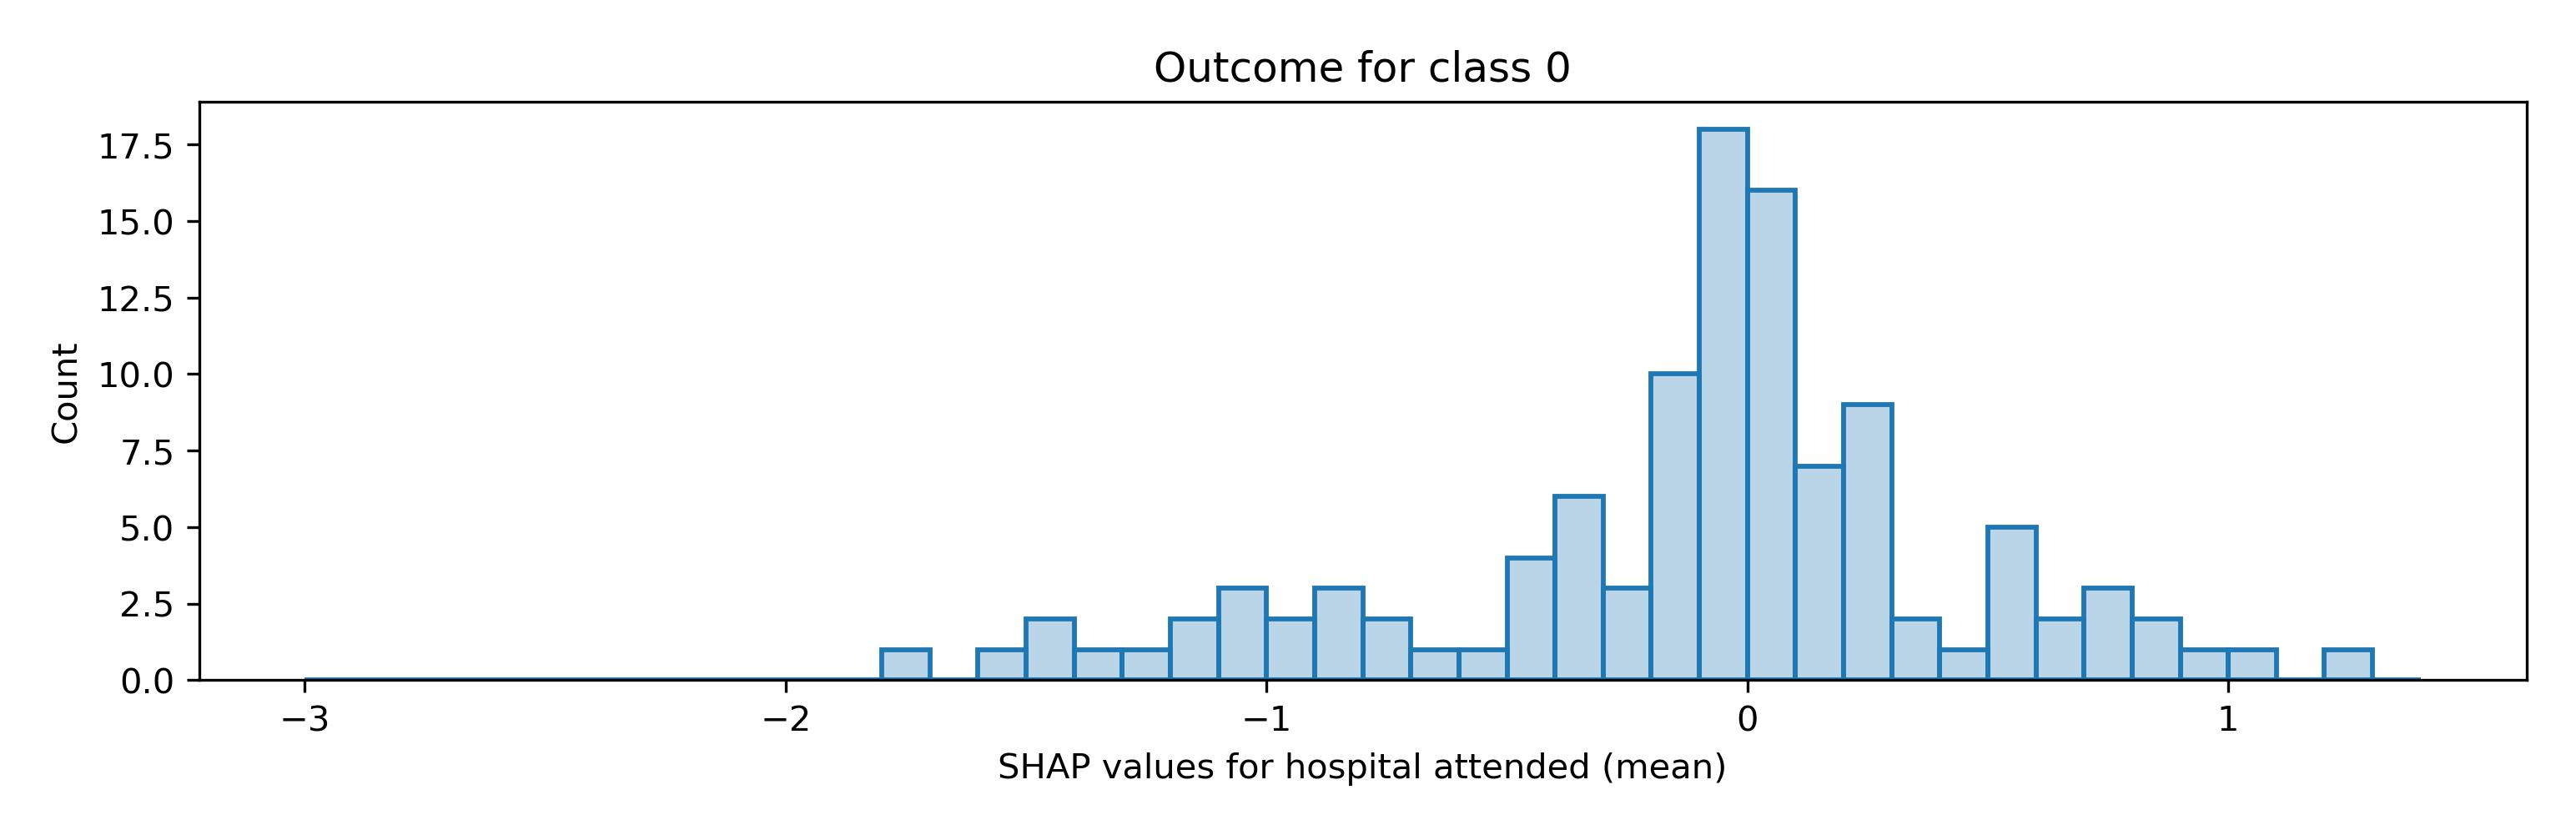
\includegraphics[trim={0 0 0 1cm}, clip, width=1\linewidth]    {./images/053_xgb_7_features_1fold_hosp_shap_hist_mrs0}\\
      \caption{\footnotesize{SHAP values for the likelihood of no disability on discharge (mRS 0). Base SHAP value = -0.405}}
      \label{fig:mrs0_violin}
    \end{subfigure}%ults
    \begin{subfigure}{.5\textwidth}
      \centering
      \captionsetup{width=.9\linewidth}
      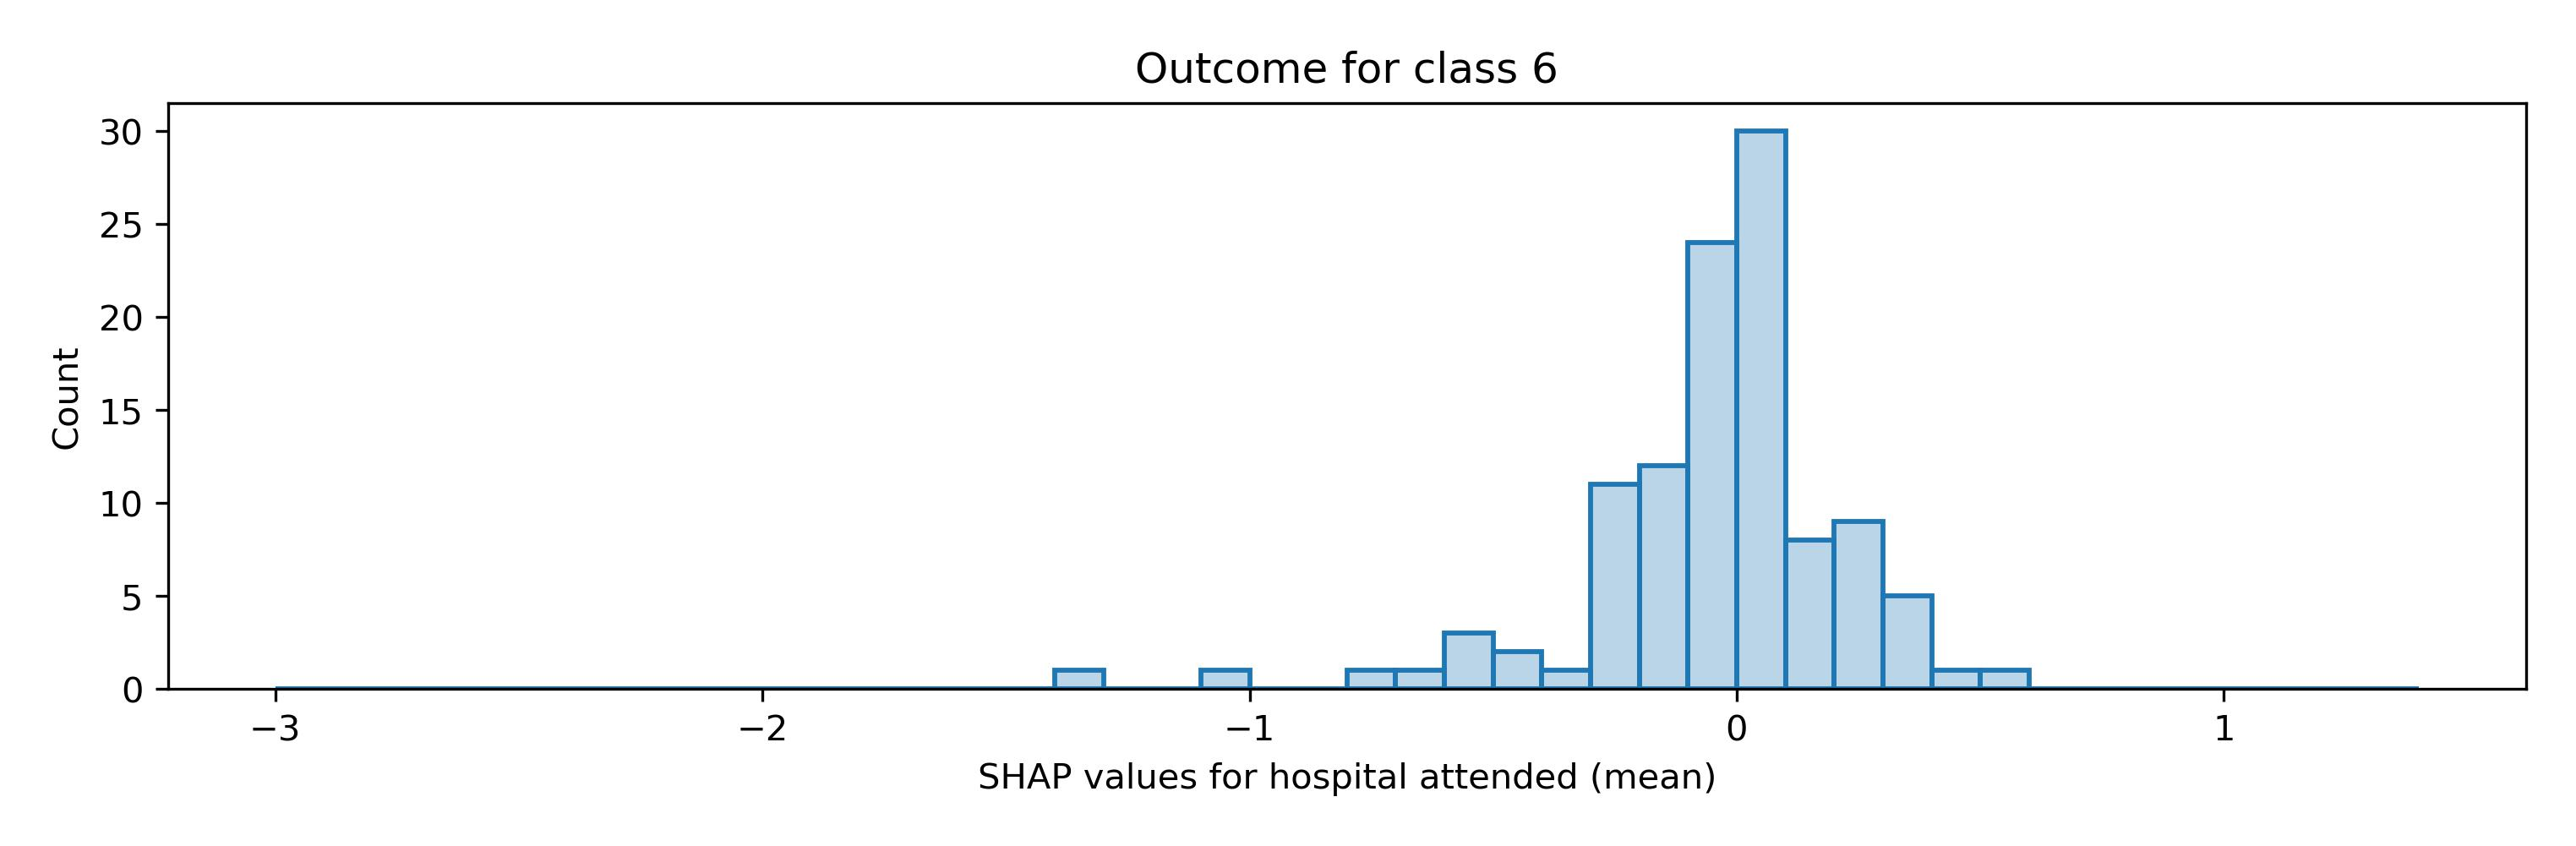
\includegraphics[trim={0 0 0 1cm}, clip, width=1\linewidth]
        {./images/053_xgb_7_features_1fold_hosp_shap_hist_mrs6}\\
      \caption{\footnotesize{SHAP values for the likelihood of death at discharge (mRS 6). Base SHAP value = -0.311}}
      \label{fig:mrs6_violin}
    \end{subfigure}
  \caption{Plots showing the relationship between SHAP values and feature values for best or worse possible outcomes. Left: Predicting the likelihood of having no disability at discharge (mRS 0). Right: Predicting the likelihood of being dead at discharge (mRS 6). Top: Violin plots showing the relationship between SHAP values and feature values. The horizontal line shows the median SHAP value. Bottom: Histogram showing the frequency of the mean SHAP value for the hospital attended.}
    \label{fig:shap_outcome_model}
\end{figure}






\textbf{Thrombolysis: Are the results from the clinical trial meta-analysis seen in real life outcomes?} \cite{pearn_thrombolysis_2024}}


\begin{itemize}
    \item Thrombolysis was found to be associated with a statistically significant improvement in the odds of having a good outcome using any mRS threshold. Regression analysis predicted a maximum 2.5-fold improvement in odds of achieving mRS 0-1, with a decline to no treatment effect at 5 hours 28 minutes post-onset. The observed beneficial effect is very similar to Emberson’s meta-analysis \cite{emberson_effect_2014} of a maximum 2.0-fold improvement in odds of achieving mRS 0-1, with a decline to no treatment effect at 6 hours 18 minutes post-onset.
    
\end{itemize}

\begin{figure}[h]
    \centering
    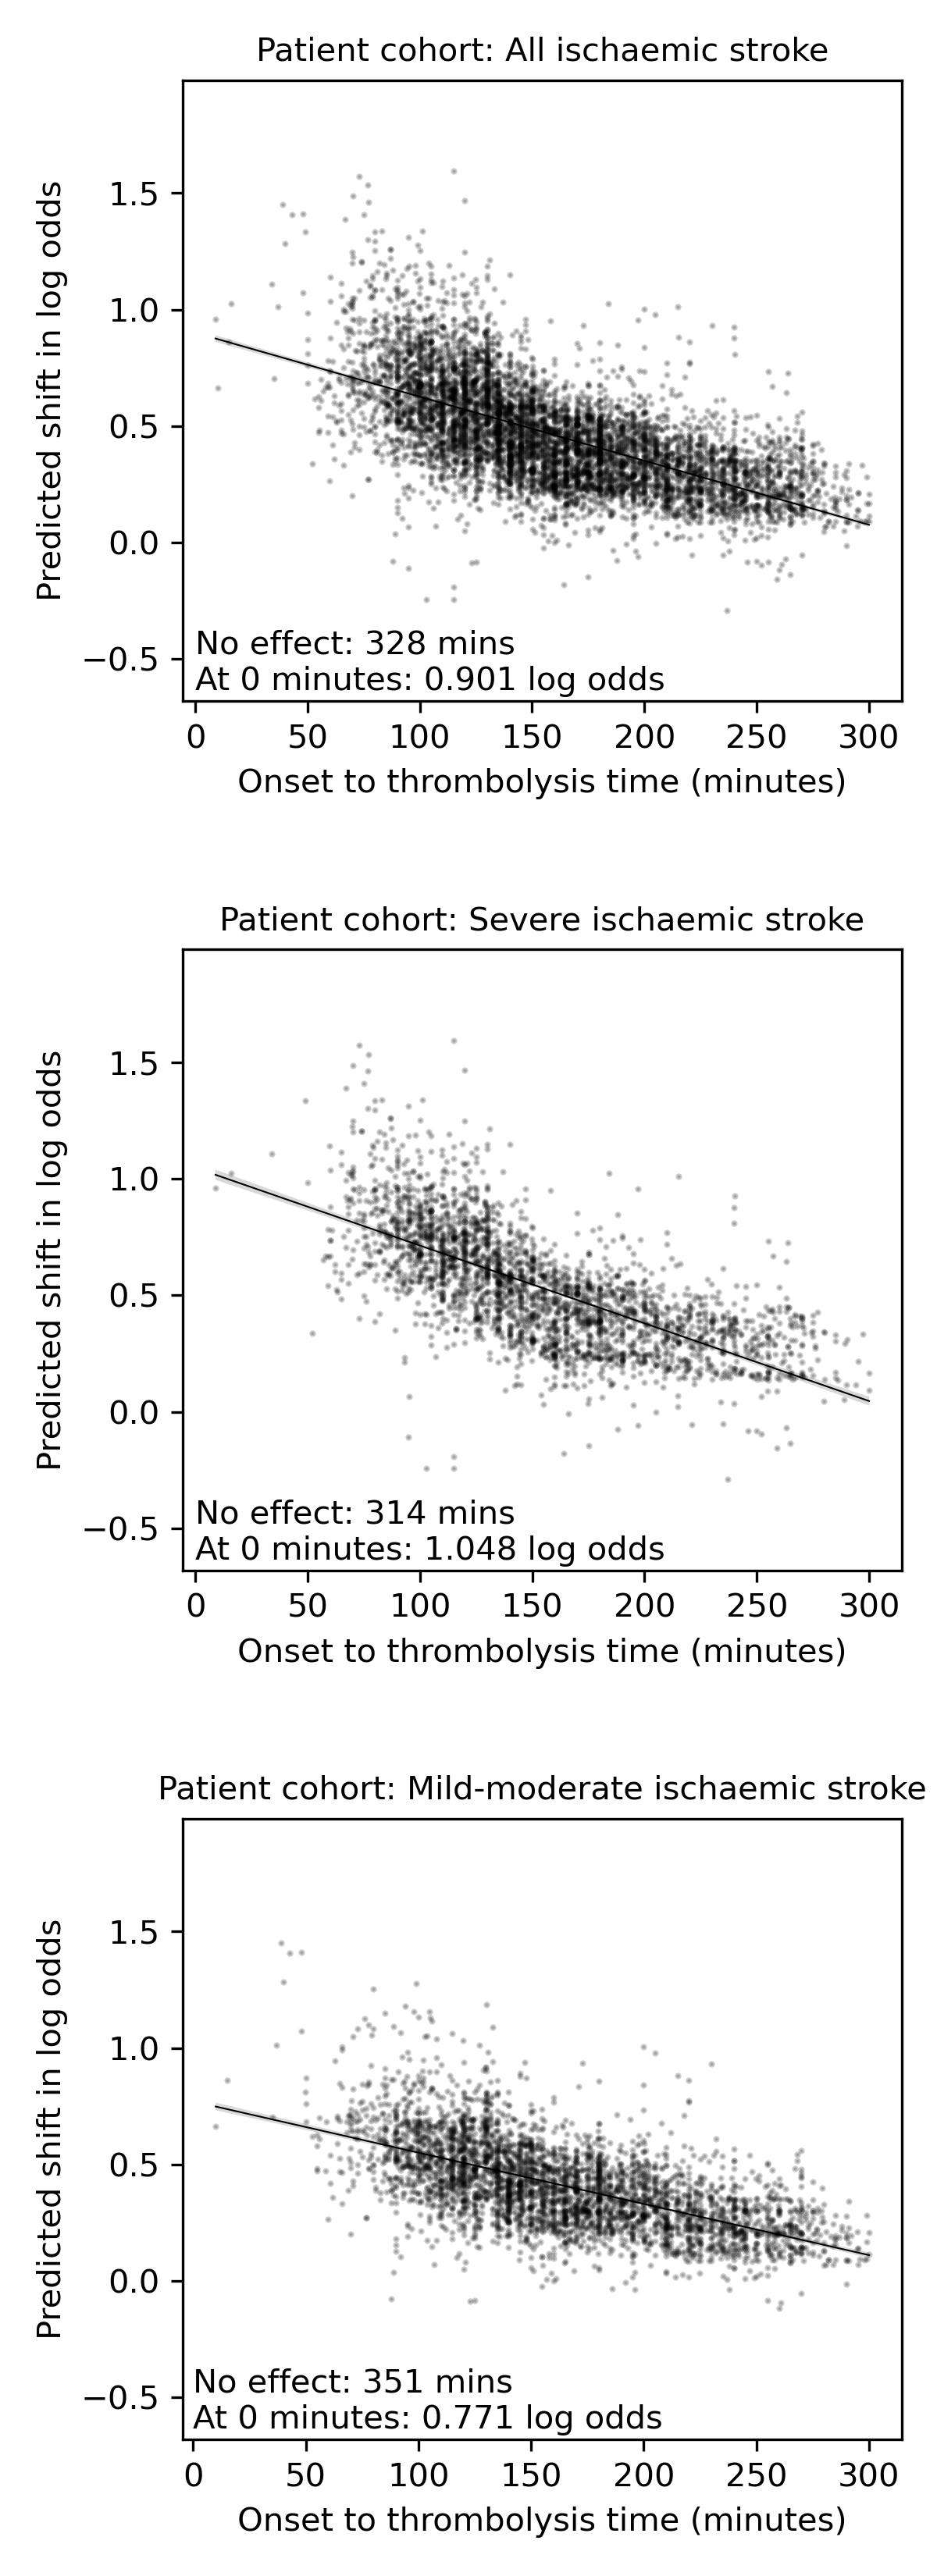
\includegraphics[width=0.40\textwidth]{./images/p3_regression_v1}\\
    \caption{A linear regression fit to the contribution from receiving thrombolysis in having a good outcome (mRS 0-1) at discharge, with respect to the onset to thrombolysis time (for patients treated within 300 minutes). Top: all treated stroke patients (n = 6,796); Middle: treated severe stroke patients, NIHSS 11+ (n = 2,856); Bottom: treated mild-moderate stroke patients, NIHSS 0-10 (n = 3,940).}
    \label{fig:linear_regression_plots}
\end{figure}

\newpage
\begin{table}[H]
    \caption{Fitting linear regression to the shift in the contribution from receiving thrombolysis towards having a good outcome (mRS 0-1) at discharge with respect to the onset to thrombolysis (OTT) time. Linear regression statistics for different patient cohorts. We used NIHSS 0-10 to define mild-moderate strokes, and NIHSS 11+ to define severe strokes.}
    \centering
        \begin{tabular}{lllllllll}
        \toprule
         Ischaemic stroke type & Variables & coef & std err & t & P$>$$|$t$|$ & [0.025 & 0.975] \\ 
         \midrule
        All & Constant & 0.9012 & 0.007 & 132.519 & 0.000 & 0.888 & 0.915\\
        & OTT time (min) &  -0.0027  & 4.04e-05 & -68.058 & 0.000 & -0.003 & -0.003\\   
        \midrule
        Severe & Constant & 1.0476  &    0.011  & 96.746 & 0.000 & 1.026 & 1.069\\
        & OTT (mins) & -0.0033 &  6.67e-05  & -50.042 & 0.000 & -0.003 & -0.003\\ 
        \midrule
        Mild-moderate & Constant &           0.7708 &     0.008   & 97.613 & 0.000 & 0.755 & 0.786\\
        & OTT time (mins) &  -0.0022 &   4.57e-05 & -48.109 & 0.000 & -0.002 & -0.002\\
        \bottomrule
        \end{tabular}
      \label{fig:stats_table_mrs1}
\end{table}


%%%%%%%%%%%%%%%%%%%%

\textbf{Are the patients who would benefit from thrombolysis the same ones as those receiving it? \cite{pearn_are_2024}}

\textbf{Key findings}

\begin{itemize}
    \item 44\% of the study population received thrombolysis. 60\% of the study population were predicted to benefit from thrombolysis (improved probability-weighted mRS and reduced probability of mRS 5-6).
    
    \item 73\% of those treated were predicted to have a better outcome with thrombolysis, and 49\% of those not treated were predicted to have a better outcome with thrombolysis.
    
    \item Patients with mismatched treatment decisions (actual thrombolysis use vs. predicted to benefit) cannot be identified from any one isolated feature value (such as stroke severity).
    
    \item Individual hospitals vary in balancing maximising benefit from thrombolysis vs. avoiding any possible harm.
\end{itemize}

\begin{figure}
\centering
    \begin{subfigure}{.7\textwidth}
      \centering
      \captionsetup{width=.9\linewidth}
      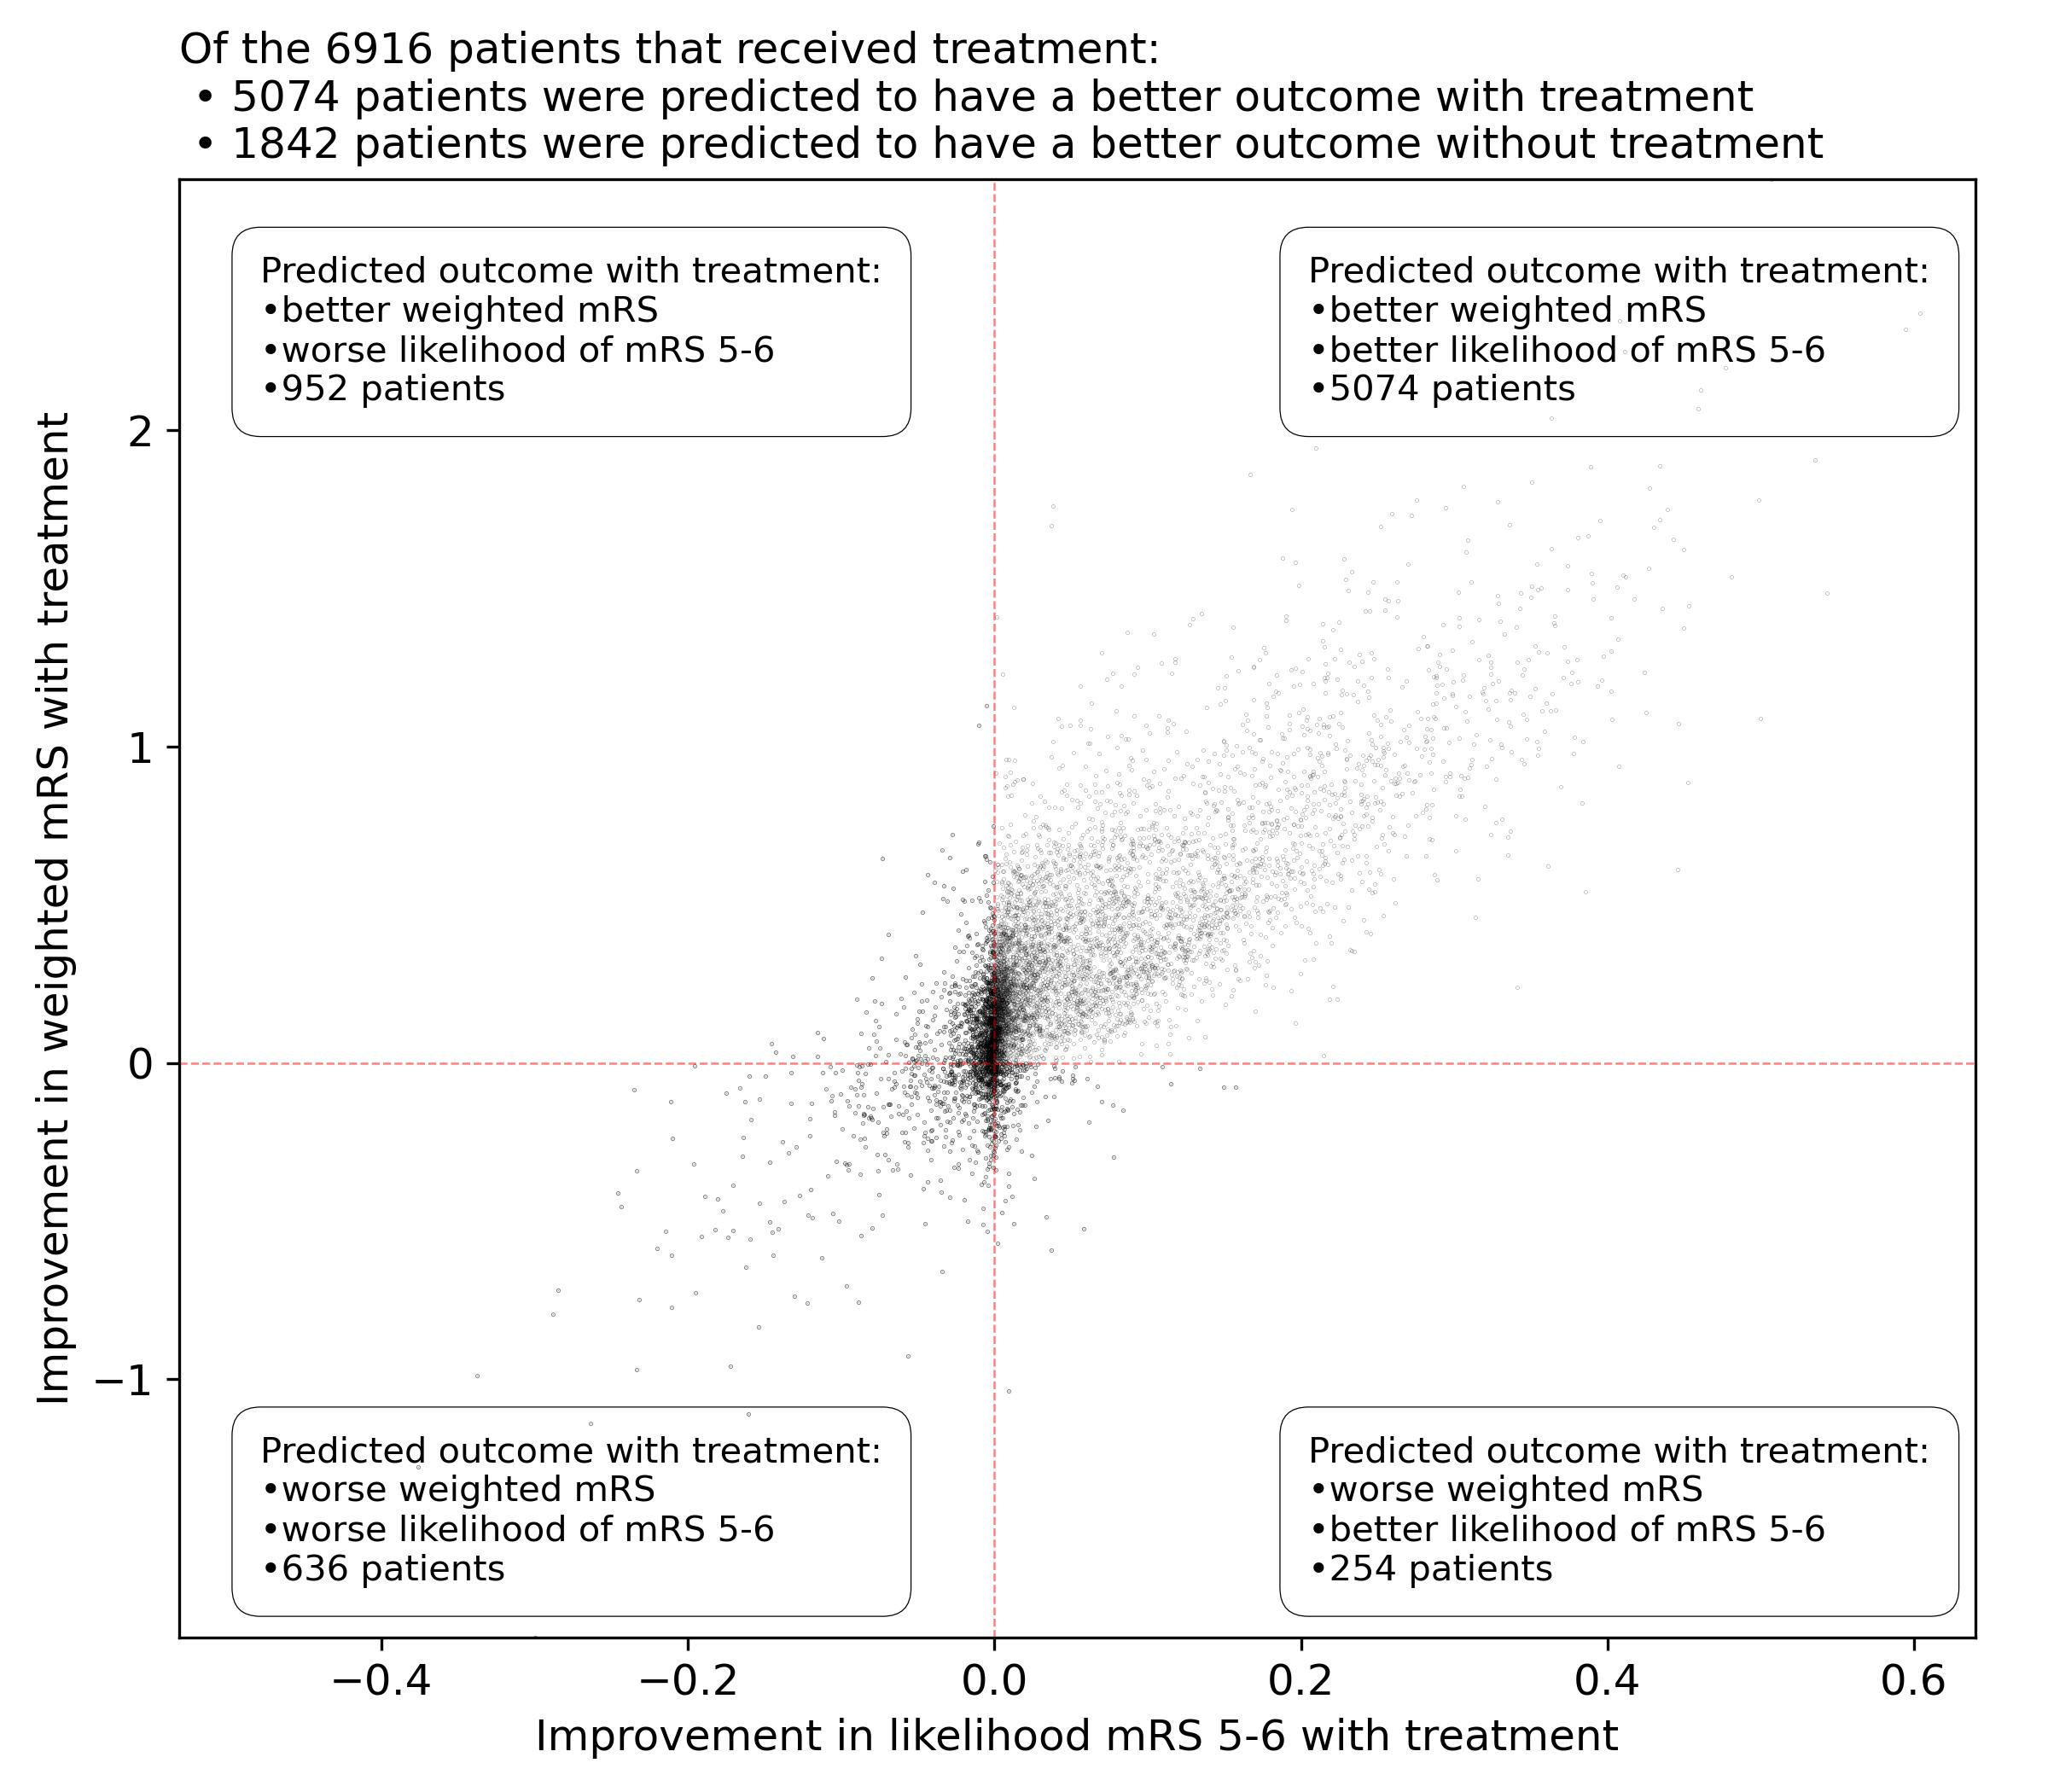
\includegraphics[trim={0 0 0 1.7cm}, clip, width=1\linewidth]{./images/p4_scatter_treated}
      \caption{\footnotesize{Patients who received thrombolysis (n = 6,916)}}
      \label{fig:scatter_receive}
    \end{subfigure}
    
    \vspace{5mm}
    
    \begin{subfigure}{.7\textwidth}
      \centering
      \captionsetup{width=.9\linewidth}
      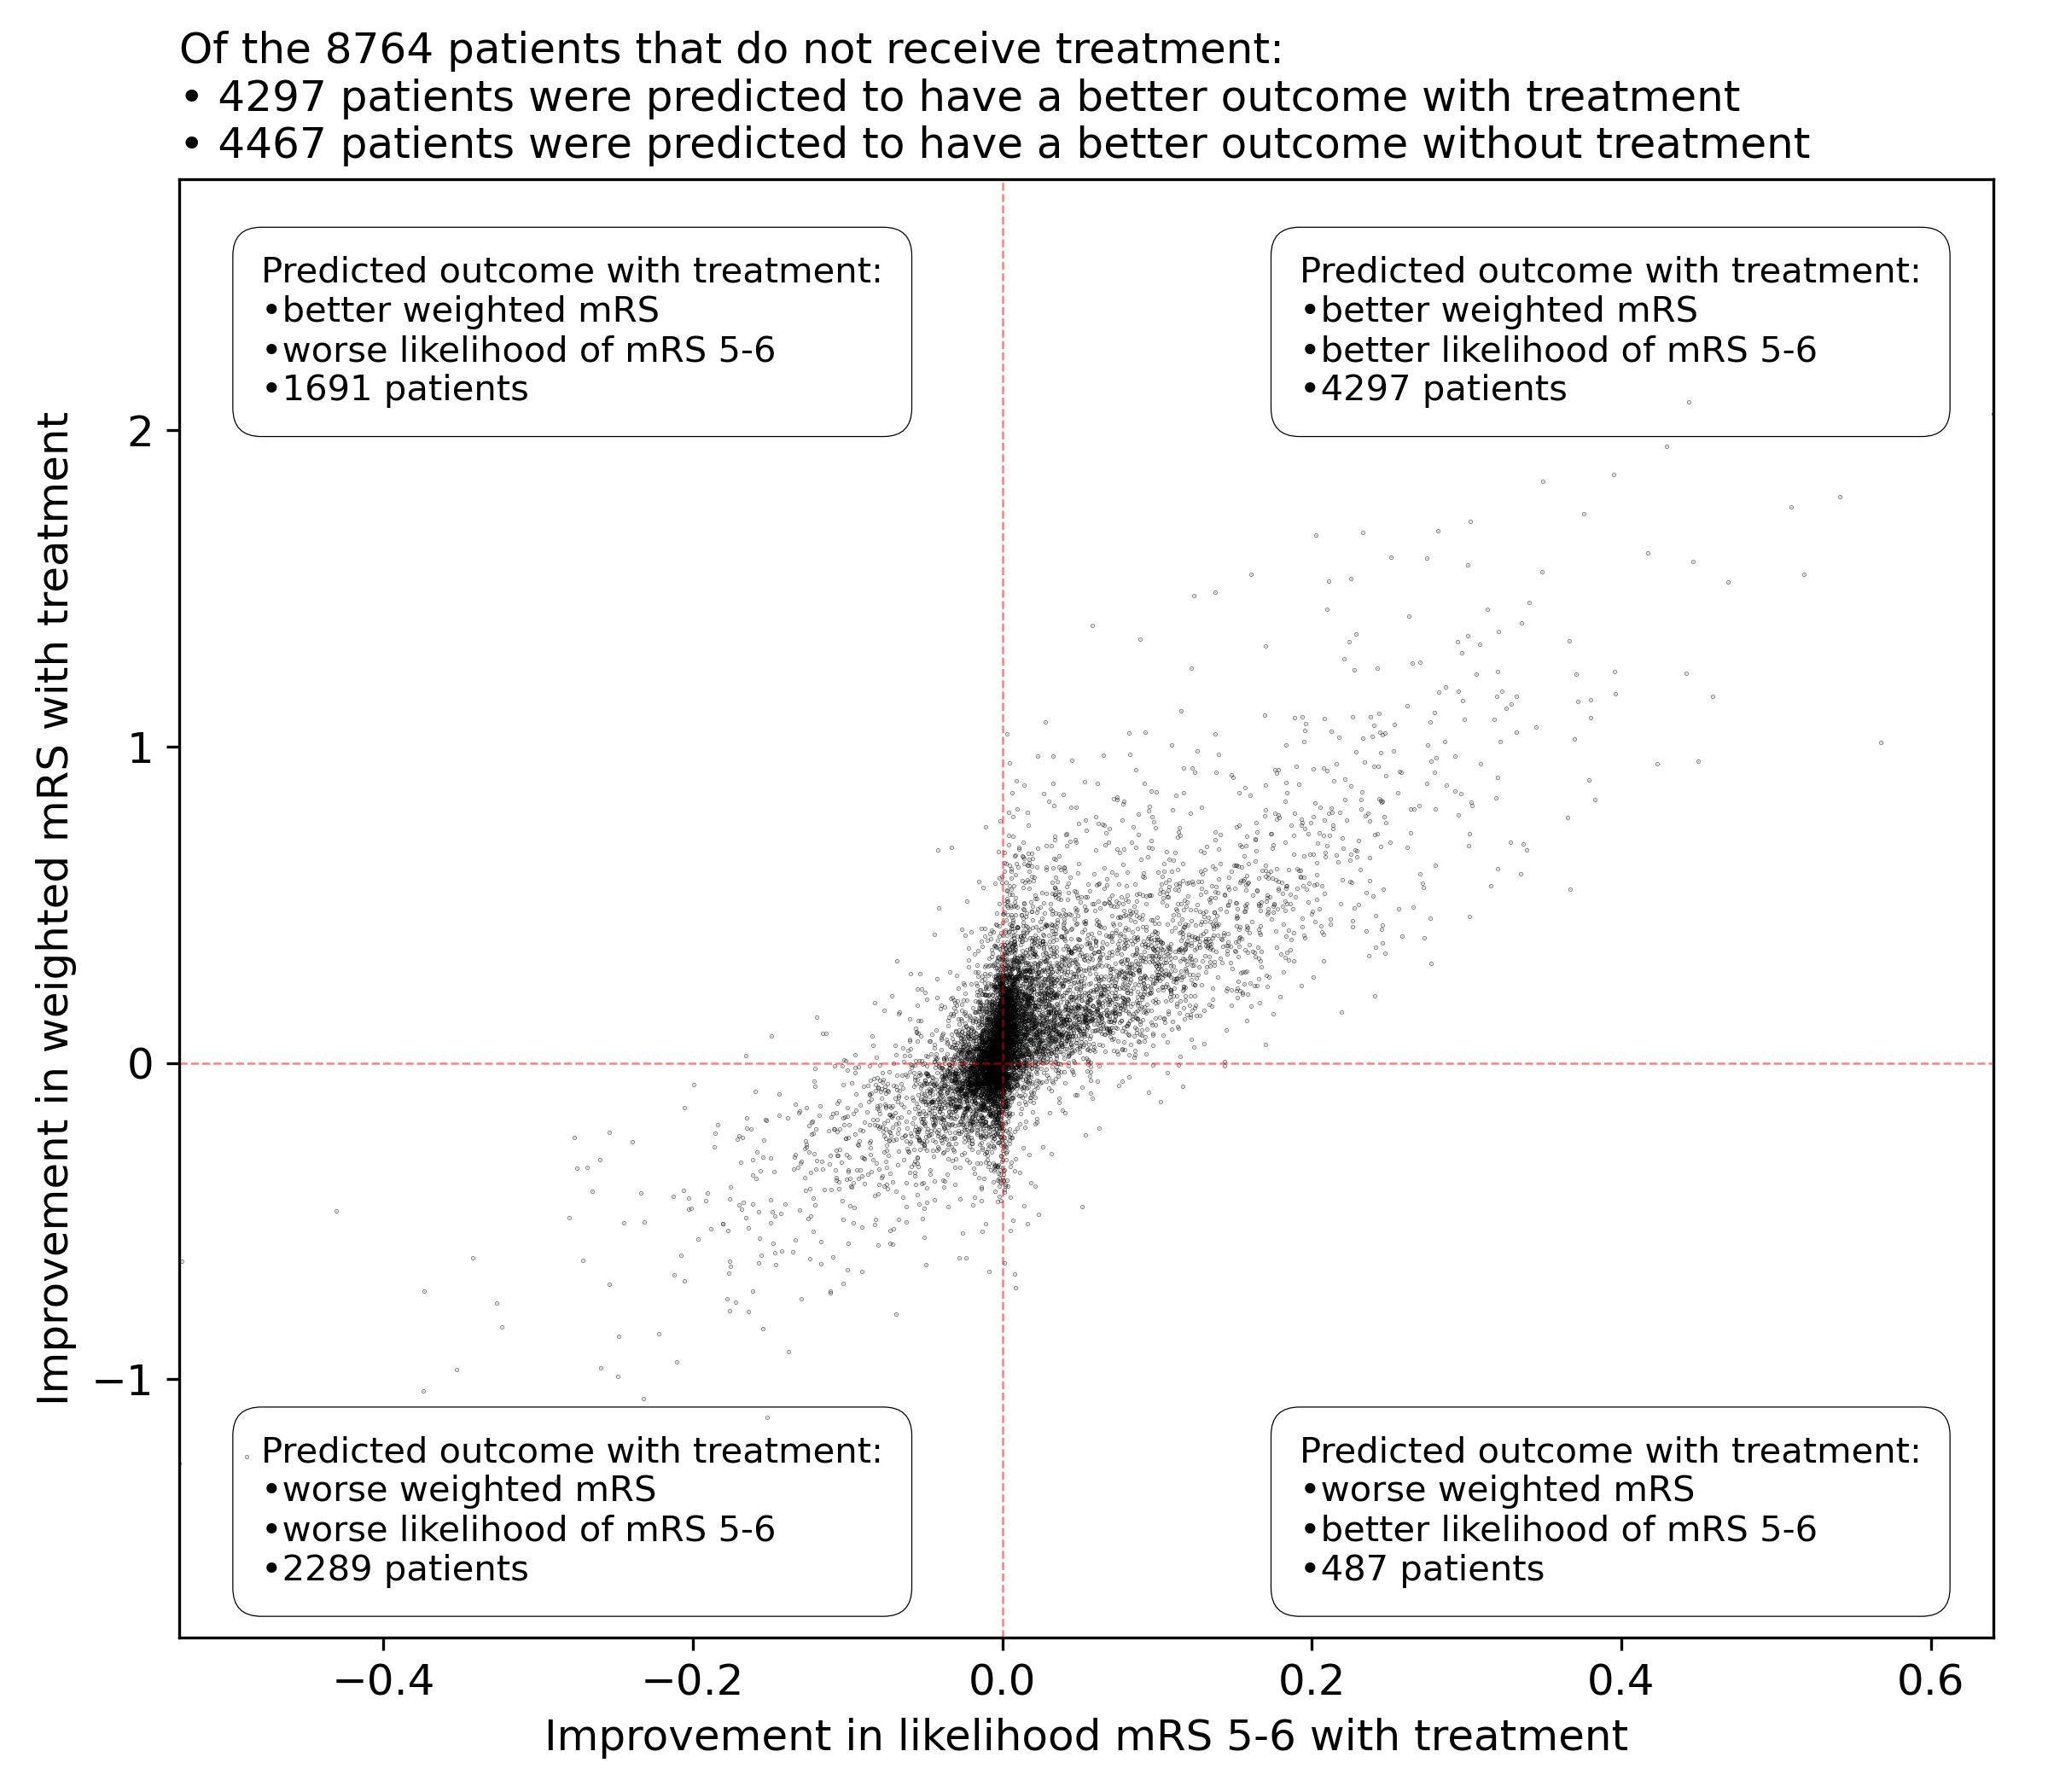
\includegraphics[trim={0 0 0 1.7cm}, clip, width=1\linewidth]{./images/p4_scatter_not_treated}
      \caption{\footnotesize{Patients who did not receive thrombolysis (n = 8,764)}}
      \label{fig:scatter_not_receive}
    \end{subfigure}
  \caption{The predicted benefit or disbenefit of thrombolysis for each of the 15,680 patients in the first k-fold test set. Benefit is shown as both the expected improvement in probability-weighted disability (y-axis) and the improvement in likelihood of avoiding discharge with mRS 5-6. Both measures are expressed so that a positive value is better (a reduction in probability-weighted disability or a reduction in probability of discharge with mRS 5-6). (a) Patients who did actually receive thrombolysis (n = 6,916), (b) Patients who did not actually receive thrombolysis (n = 8,764).}
\label{fig:scatter_all}
\end{figure}

\begin{figure}
    \centering
    {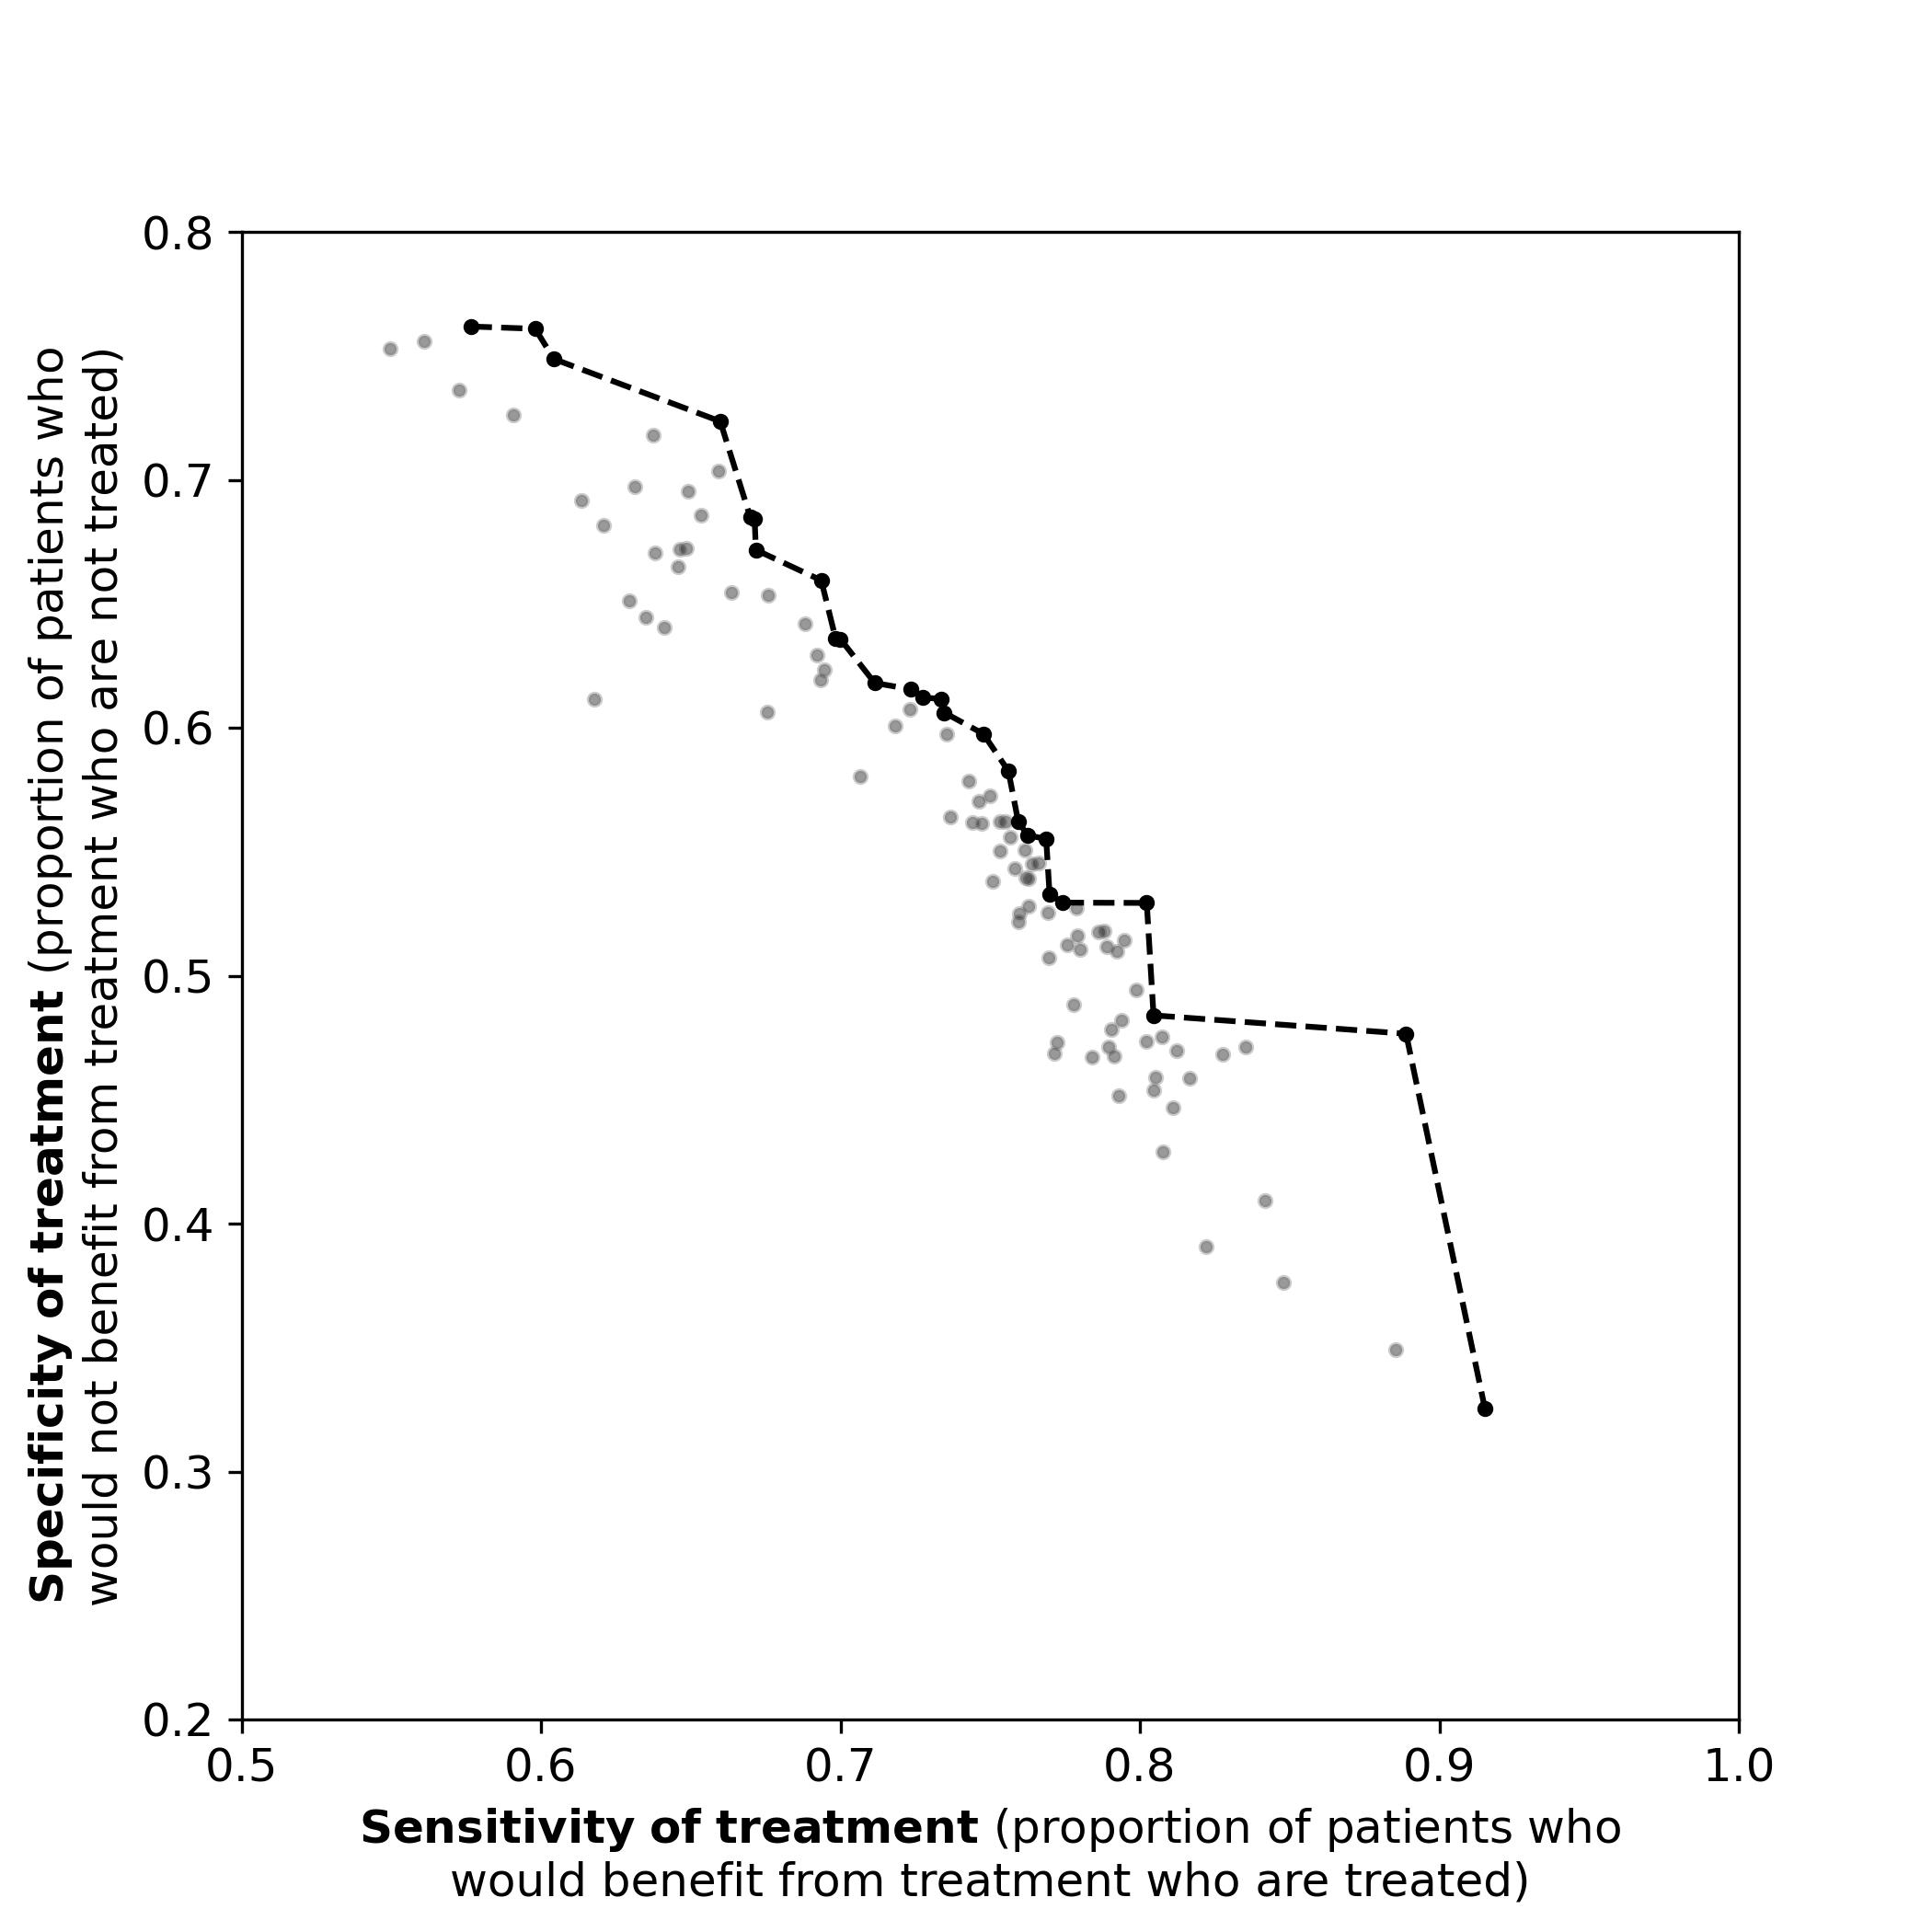
\includegraphics[width=0.65\linewidth]{./images/p4_spec_sens}} 
    \caption{\textit{Sensitivity} (proportion of patients who were predicted to benefit from thrombolysis who were predicted to receive thrombolysis) and \textit{specificity} (proportion of patients who were predicted \textit{not} to benefit from thrombolysis who were predicted \textit{not} to receive thrombolysis) for each stroke team. The dotted line shows the hospitals on the Pareto front where there are no hospitals that have a better \textit{sensitivity} without a worse \textit{specificity}, or vice-versa.}
    \label{fig:hosp_shap_scatter}
\end{figure}